\label{sec:meshoperations}
\subsection{Representation Deficit}
The concept of representation deficit was discussed in \cite{mclaurin13}
in the context of scale-independent measure of curve discretizations.
Here, the concept will be extended to two dimensions. It is important
that any criteria for refinement maintain scale indepdence. This is so
that the values for representation deficit can be compared between
different candidate operations. Below, representation deficit is defined
and discussed for four fundamental mesh operations: triangle split, edge
split, edge swap, and node smoothing.

\subsection{Triangle Split}
A triangle is a planar object, and is representing a possibly non-planar
portion of a surface. Any triangle, with area $A_T$, in the
discretization can have at most the same area as the portion of the
surface which it represents, $A_S$. Therefore, the representation
deficit for a triangle, $RD_T$, is defined as $RD_T = \frac{A_S -
A_T}{A_T}$. Note that the areas are calculated in ${\mathbb R}^3$. The
difference in surface area, $\left(A_S - A_T\right)$, is normalized by
$A_T$ so that the result is scale independent. Also, this is a
representation {\it deficit} since $A_S \ge A_T$ is always true.

In order to apply the above definition of representation deficit to a
mesh generation, a replacement for $A_S$ must be determined since the
area of the surface represented by $A_S$ is not always able to be
determined---or, most often, the area calculation is impractical.
Generally, in order to reduce the representation deficit for a triangle
the triangle is split by inserting an interior point. Any point that is
inserted into the interior of the triangle would decrease the
representation deficit---or at worst it will remain the same. However,
the determination of where to split the triangle should be done in such
a way that the representation deficit is minimized. This strategy of
refinement, refining each triangle in such a way that the representation
deficit is locally minimized, would take advantage of the optimal
substructure the discrete topology.

\begin{figure}[h!]
  \center{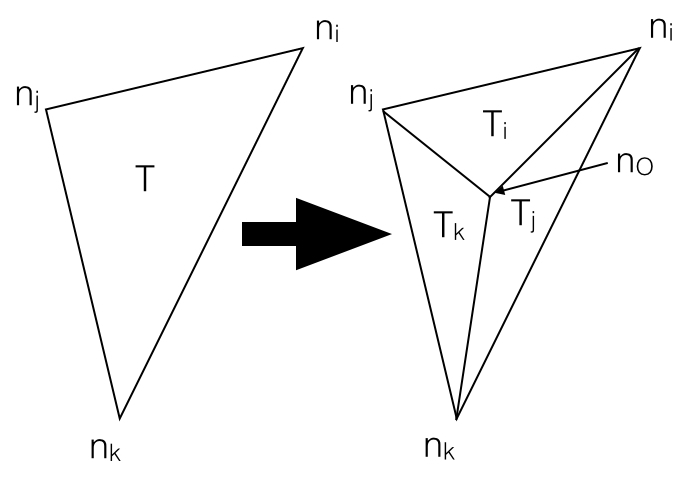
\includegraphics[height=1.4in]
    {Figures/TriangleSplit.jpg}}
  \caption{Triangle Split}
\end{figure}

The process of determining where to split a triangle is defined here by
a locally optimizing an objective function defined for a triangle: Let
$S(u,v)$ be a parameterized surface, $D$ be be a discretization of the
surface, and $T$ be a triangle (included in $D$) defined by an ordered
tuple of nodes, $\left(n_i, n_j, n_k\right)$. These nodes are ordered
such that the triangle normal is positive. Specifically, if $\vec{V_0} =
\left\{n_j - n_i \right\}$ and $\vec{V_1} = \left\{n_k - n_i\right\}$
then the triangle normal, $N_T = \vec{V_0} \times \vec{V_1}$, is
positive. Note that a two-dimensional cross-product (or two-dimensional
curl) is a scalar quantity. Additionally, let a node on the interior of
$T$ be defined as $n_O$. The four nodes, $n_i$, $n_j$, $n_k$, and $n_O$
define three triangles, $T_i\left(n_i,n_j,n_0\right), T_j\left(n_j, n_k,
n_0\right), T_k\left(n_k, n_i, n_0\right)$. If $A(T)$ is a function
that calculates the area of a triangle in $\left(x,y,z\right)$ space,
then the optimization problem for finding the optimal position for $n_0$
in $T$ is defined as:

\begin{eqnarray*}
\begin{array}{rcl}
\underset{n_O}{\text{minimize}} \ O(T) & = & - \frac{A\left(T_i\right) + A\left(T_j\right) + A\left(T_k\right) }{ A\left(T\right) }\\
\text{subject to} \ N_{T_i} & > & 0 \\
N_{T_j} & > & 0 \\ 
N_{T_k} & > & 0. \\
\end{array}
\end{eqnarray*}

It should be noted that this definition of representation deficit would
be difficult to derive or express for a topological entity other than a
triangle. This is due to the inherent ambiguity in the definition of not
only the surface area, but also the surface representation of (possibly)
non-planar elements, e.g. non-planar, or skew, quadrilateral. [MORE
POSSIBLY]

\subsection{Edge Split}
An edge in parametric space represents a (possible) curve on the
surface. Any edge, with length $L_E$, can have at most the same length
as the portion of the surface which it represents, $L_S$. Therefore, the
representation deficit for an edge, $RD_E$, is defined as $RD_E =
\frac{L_S - L_E}{L_E}$. Note that the lengths are calculated in
${\mathbb R}^3$. The difference in length, $\left(L_S - L_E\right)$, is
normalized by $L_E$ so that the result is scale independent. Also, this
is a representation {\it deficit} since $L_S \ge L_E$ is always true;

In order to apply the above definition of representation deficit to mesh
generation, a replacement for $L_S$ must be determined since the length
along the surface represented by $L_S$ is not always able to be
determined -- or, most often, the arc-length calculation is impractical.
Generally, in order to reduce the representation deficit for an edge the
edge is split by inserting an interior point. Any point that is inserted
into the interior of the edge would decrease the representation deficit
--- or at worst it will remain the same. However, the determination of
where to split the edge should be done in such a way that the
representation deficit is minimized. This strategy of refinement,
refining each edge in such a way that the representation deficit is
locally minimized, would take advantage of the optimal substructure of
the discrete topology. A method for generating a locally optimal edge
split is detailed in \cite{mclaurin12,mclaurin13}[OTHERS].

\begin{figure}[h!]
  \center{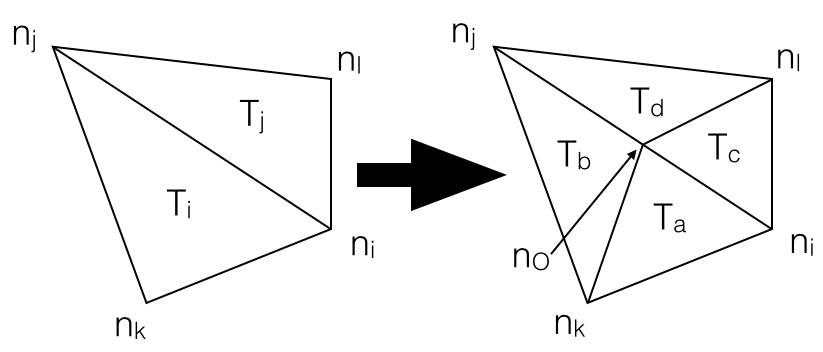
\includegraphics[height=1.4in]
    {Figures/EdgeSplit.jpg}}
  \caption{Edge Split}
\end{figure}

In addition, the fact that an edge split will change the surface area of
the discretization should be considered. Since the overall justification
of this work is reduce the {\it area} representation deficit of a
discretization, the representation deficit will not be defined for an
edge but for an edge-split. Therefore, for a given edge, only the
edge-split that minimizes {\it area} representation deficit is
considered. The process of determining where to split a triangle is
defined here by locally optimizing an objective function defined for an
edge-split.  Let $E\left(n_i,n_j\right)$ be an edge in $D$ that is
topologically adjacent to two triangles, $T_i\left(n_i,n_j,n_k\right)$,
and $T_j\left(n_i,n_l,n_j\right)$. Additionally, let a node on the
interior of the edge be defined as $n_O$. The five nodes,
$\left\{n_i,n_j,n_k,n_l,n_O\right\}$ define four triangles,
$T_a\left(n_i,n_O,n_k\right)$, $T_b\left(n_O,n_j, n_k\right)$,
$T_c\left(n_i,n_l,n_O\right)$, $T_d\left(n_O,n_l,n_j\right)$.  The
optimization problem for finding the optimal position for $n_O$ on $E$
is defined as:

\begin{eqnarray*}
\begin{array}{rcl}
\underset{n_O}{\text{minimize}} \ O(E) & = & - \frac{ A\left(T_a\right) + A\left(T_b\right) + A\left(T_c\right) + A\left(T_d\right) }{ A\left(T_i\right) + A\left(T_j\right) } \\
\text{subject to} \ N_{T_a} & > & 0 \\
N_{T_b} & > & 0 \\ 
N_{T_c} & > & 0 \\
N_{T_d} & > & 0. \\
\end{array}
\end{eqnarray*}

% NOTE:  I suggestion we rename this subsection.  Whenever optimization is 
%   used, the term smoothing is no longer used, as smoothing can lead
%   to a decrease in the metric being measured.  With mesh quality, the 
%   appropriate term is mesh quality improvement.  I would have used the 
%   term mesh representation deficit improvement here.  However, since
%   this is a subsection and all subsection titles should be parallel,
%   that doesn't quite work either.  Can you think of a better title?

\subsection{Nodal Smoothing}
In this paper, the focus is on using nodal smoothing in 
order to locally minimize the representation deficit in the surface mesh.  
It should be noted that, although a locally optimal mesh topology could 
also be obtained, computing such a topology would involve the solution of 
a discrete optimization problem (via integer programming) which would 
specify the relevant sequence of edge flips.  The discrete 
and continuous optimization problems could then be solved in an iterative, 
interleaving fashion.  However, such an approach would require significant 
additional computational expense.

For a node, $N_i$, the representation deficit is defined only by
comparing it to the node when located at another point in space. Here
the comparison is bound by limiting the range of comparison within the
edge-hull topologically adjacent to $N_i$. Formally, let $N_i$ be a node
in $D$ that is shared topologically by $n$ triangles, where $n$ is the
face-valence of $N_i$. The optimization for finding the optimal position
for $N_i$ is defined as:

\begin{eqnarray*}
\begin{array}{rcl}
\underset{N_O}{\text{minimize}} \ O(N) & = &
-\sum{_{j=1}^{n_t-1}A\left(T_j\right)} \\
\text{subject to} \ N_{T_1} & > & 0 \\
N_{T_2} & > & 0 \\ 
N_{T_3} & > & 0 \\
& \vdots & \\
N_{T_{n-1}} & > & 0 \\ 
N_{T_n} & > & 0.
\end{array}
\end{eqnarray*}

\begin{figure}[h!]
  \center{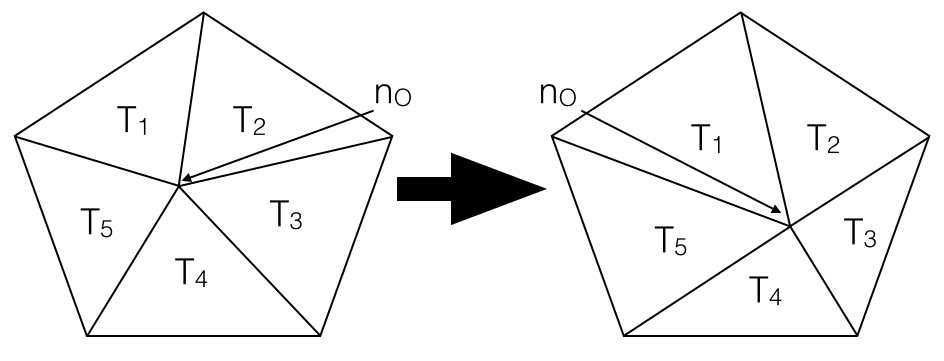
\includegraphics[height=1.4in]
    {Figures/NodalSmoothing.jpg}}
  \caption{Nodal Smoothing}
\end{figure}

[NEED TO DISCUSS HESSIAN/METRIC BASED MESH ADAPTION IN THE NODAL
SMOOTHING SECTION OF THE PAPER. THERE IS NO GLOBAL, STATIC FUNCTION
AGAINST WHICH THE INTERPOLATION ERROR CAN BE MINIMIZED. THAT IS,
WHENEVER THE MESH MOVES, THE INTERPOLATION ERROR FIELD CHANGES.]


%\subsection{Boundary Refinement}
%[Is there a section needed on this? It'd be straightforward to talk about
%but would be pretty repetitive and I don't have it coded up yet. If I do
%talk about it then due diligence says I should show some results and
%there are already tons of variables to consider. This might get left out
%due to space concerns.]
%[This should be an argument for applying [CITE SELF] to the boundary
%curves first because the interior of the surface is not what the
%boundary curves are really trying to represent]
